\chapter{Wolterミラー評価実験の手法に関する検討}
\thispagestyle{empty}
\label{chap3}
\graphicspath{{chap3/figure/}}
\minitoc

\newpage
%%%%%%%%%%%%%%%%%%%%%%%%%%%%%%%%%%%%%%%%%%%%%%%%%%%%%%%%%%%%%%%%%%%%%%%%%%%%%


% ================================================== %
% section
% ================================================== %
\section{諸言}
\label{chap3_introduction}

\ref{chap2}章では、Wolterミラーの誤差応答シミュレーションを行い、各種形状誤差によって生じる波面誤差分布を計算した。
本研究の目的であるミラー上の形状誤差量の測定は、それぞれの誤差に対応する波面誤差分布を基底としてミラー下流端面における波面を分解することによってなされる。
本章では、波面計測に用いる位相回復法について基礎的な理論を述べた上で様々な手法について検討し、計測に用いる手法を決定、提案する。
また、提案された手法について測定対象の天文用Wolterミラーに合わせたシミュレーションを行い、その有効性を確認する。

\clearpage
% ================================================== %
% section
% ================================================== %
\newpage

\section{手法の決定に関する方針}
\label{chap3_method_choice_policy}

本節では、手法の検討に先立って、計測方法に対して要請される事項について述べる。

\subsection{高空間分解能}
\label{chap3_high_spatial_resolution}
1章で述べたように、測定対象となるWolterミラーで波面計測を行う際の大きな問題点は、2回反射されたビームが非常に細い輪帯形状をなすことである。
この極めて細い輪帯波面を測定し、形状誤差の情報を計算するためには、形状誤差が波面の動径方向に与える変化を十分な空間分解能で計算できなければならない。
当然、動径方向分解能が高くなるほど長手方向の形状誤差の位置分解能も上がるが、ここでは最低限の条件として3次のコマ収差を検出できること、すなわち動径方向に3画素の分解能を持つことを要請として定める。

\subsection{ダイナミックレンジ}
\label{chap3_dynamic_range}

位相回復計算を行う上で非常に重要な要素の1つが、カメラのダイナミックレンジである。
測定する強度分布において一定値を下回る点では強度が0として検出されてしまうため、同じ強度分布を持つ系であっても回復計算に対して有効な領域はダイナミックレンジによって左右される。
逆に、同じダイナミックレンジに対して有効な領域の大小によって回復計算の収束性や得られる情報の質が変化する。
本研究で用いるCCDカメラのパラメータは表\ref{tb:ccd_camera_params}の通りであり、これに対して回復計算が実行できるような手法であることが要請される。

\begin{table}[!ht]
\begin{center}
  \caption{CCDカメラのパラメータ}
  \begin{tabular}{|c|c|l|} \hline
    項目 & 値 \\ \hline
    製品名 & Bitran BQ-85M \\
    ピクセルサイズ & 9.0 um \\
    画素 & 4096 $\times$ 4096 \\
    受光面積 & 36.9 mm $\times$ 36.9 mm \\
    A/Dコンバータ & 16bit (65535階調) \\ \hline
  \end{tabular}
  \label{tb:ccd_camera_params}
\end{center}
\end{table}

\clearpage
\newpage

% ================================================== %
% section
% ================================================== %

\section{位相回復法}

\subsection{位相回復法の概要}
\label{chap3_phase_retrieval_introduction}

1章\ref{chap1_wave_metrics}でも述べた通り、位相回復法は波面計測法の一種であり、CCDなどの受光素子で計測された強度値の情報から位相分布を算出する方法である。
より具体的には、測定対象の波面の存在する領域について、$N \times N$の強度計測値を元に$N \times N$の位相を求める。
位相回復法には様々な手法が存在するが、いずれの方法においても基本的な方針は共通している。
未知数となっている位相をすべて決定するためには、それら未知数を含む十分な本数の方程式を立式する必要がある。一般に、求める光学波動場において強度と位相の間に拘束関係はない。
そこで、測定対象の波面領域に加えて光の進行方向にもう1つ未知の波面領域を定め、これら2つの領域間での光学波動場の伝播を関係式として与えることで、求める未知数を含む方程式を得ることができる。
これを図\ref{fig:phase_retrieval_policy}に示す。
波動場の伝播は$N \times N$の離散領域に対して$N \times N$本の数式で表される。
これだけでは未知数が$3N \times N$個に対して方程式が$N \times N$本と少なく、未知数を全て決定することができない。
そこで、未知数を減らす、もしくは成立する方程式を増やすといった工夫を行うことで、解を決定するという方針を取る。

\begin{figure}[!ht]
\centering
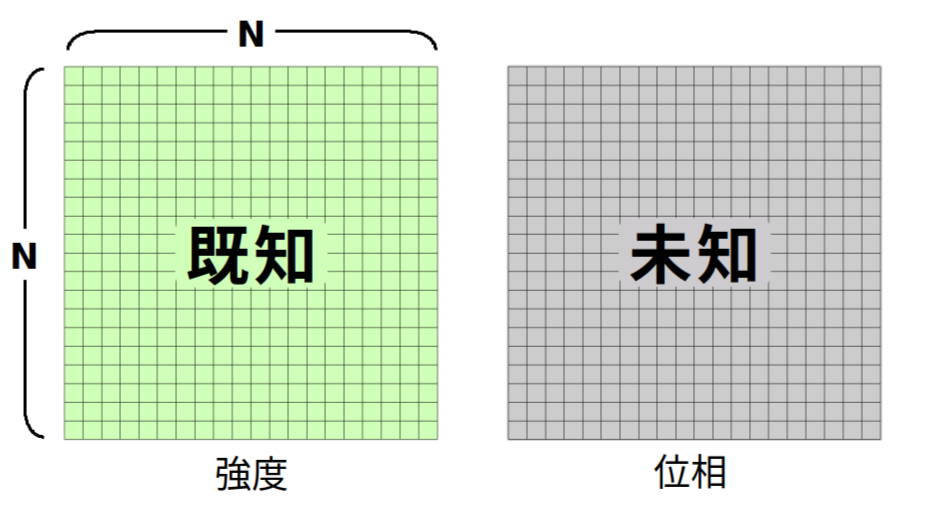
\includegraphics[width=6cm]{phase_retrieval_problem.png}
\caption{位相回復問題}
\label{fig:phase_retrieval_problem}
\end{figure}

\begin{figure}[!ht]
\centering
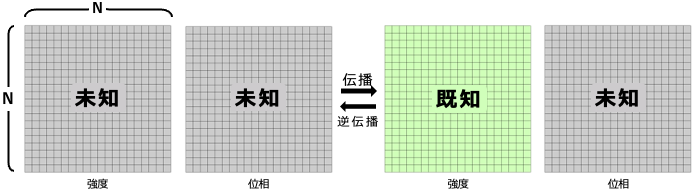
\includegraphics[width=12cm]{phase_retrieval_policy.png}
\caption{位相回復法の方針}
\label{fig:phase_retrieval_policy}
\end{figure}

2つの平面が十分遠い場合、あるいは集光前後の関係にある場合、波動場の伝播はフーリエ変換の関係で表現できることが知られている。
このことを示唆してフーリエ変換前を実空間、変換先を逆空間と呼ぶならば、位相回復計算のブロック図による表現は図\ref{fig:phase_retrieval_blockgram}のようになる。
回復計算は4段階で進行する。
まず実空間での波動場を逆空間へと伝播する。
次に、逆空間での拘束、たとえば焦点面で取得された強度分布によって強度を置き換えるなどの計算を行う。
実空間へ逆伝播したのち、利用する特定のアルゴリズムの更新則に従って波動場を更新する。

\begin{figure}[!ht]
\centering
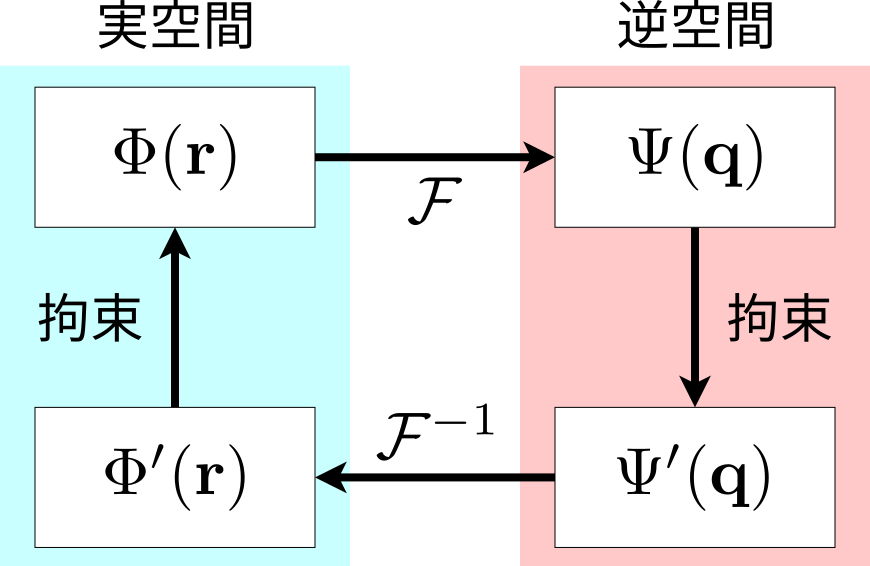
\includegraphics[width=12cm]{phase_retrieval_blockgram.png}
\caption{位相回復計算のブロック図}
\label{fig:phase_retrieval_blockgram}
\end{figure}


\subsection{サンプリング定理}
\label{chap3_sampling_theorem}

ある2つの平面の間での光波の伝播がフーリエ変換で与えられるとき、二平面はそれぞれもう一方の周波数領域(波数領域)での表現になっており、カメラで取得される離散領域に対して適用し離散フーリエ変換を行うとき、サンプリング定理によって互いに領域サイズは拘束関係にある。
逆空間の領域はナイキスト周波数$k_s$に対して$[-k_s, k_s]^2$として与えられるので、これを実空間、逆空間の空間分解能に対して表すと、式\ref{eqn:sampling_theorem_px},\ref{eqn:sampling_theorem_size}のようになる。
ただし、波長を$\lambda$、焦点距離を$f$とし、領域の1画素の一辺を$\Delta L_r, \Delta L_f$、領域全体の一辺を$L_r=N \Delta L_r, L_f = N \Delta L_f$とする。

\begin{eqnarray}
  \Delta L_{\mathrm{real}} \Delta L_{\mathrm{reciprocal}} = \frac{f  \lambda}{N} \label{eqn:sampling_theorem_px} \\
  \Leftrightarrow 
  L_{\mathrm{real}} L_{\mathrm{reciprocal}} = N f \lambda \label{eqn:sampling_theorem_size}
\end{eqnarray}

これは、ミラー下流端面における空間分解能が高い波面領域を取ることは、焦点面において広い波面領域を取ることと等価である。

\clearpage
\newpage

\subsection{孤立条件の利用}
\label{chap3_solitude_introduction}
主にCDI(コヒーレント回折イメージング)の文脈において、波動場が到達しない領域を定数0として与えることで、未知数をの総数を激減させるという方法が多く取られる。
CDIとは、図\ref{fig:cdi_schematic}に示すように、サンプルに集光ビームを照射し、その回折像を見ることでそのサンプルの内部構造を解析する方法である。

\begin{figure}[!ht]
\centering
\includegraphics[width=12cm]{cdi_schematic.png}
\caption{コヒーレント回折イメージングの概要}
\label{fig:cdi_schematic}
\end{figure}

位相回復法によってディテクターでの位相およびサンプル面における位相・強度を求めることで、サンプル各点における透過率を求めることが目標となる。
このような系においては、カメラの画素をより細かく取ることにより、対応するサンプル面での領域がサンプルより大きく広がるため、この領域には波面が存在しないという仮定を用いて回復計算を行うことができる。
Wolterミラーの計測に用いる場合は、焦点面にCCDカメラを配置し、ミラーの輪帯に対して孤立条件を適用することになる。
この方針に則って、位相回復計算を行う最もシンプルなアルゴリズムがBIO(Basic Input-Output) Algorithmである。
疑似コードをAlgorithm\ref{alg:bio}に示す。

\newcommand{\pos} {
    \mathbf{r}
}
\newcommand{\rpos} {
    \mathbf{q}
}

\begin{algorithm}                      
\caption{BIO Algorithm}         
\label{alg:bio}                          
\begin{algorithmic}
    \STATE $\phi_0(\pos)$
      = $\begin{cases}
        \mathrm{rand} & (\pos \in S) \\
        0 & (\pos \notin S)
      \end{cases}$
    \FOR{n = 0 \ldots N-1}
    \STATE $\Psi_n(\rpos) = \mathcal F [\phi_n(\pos)]$
    \STATE $\Psi_{n+1}(\rpos) = \sqrt{I(\rpos)} \exp \left( i \arg \Psi_n(\rpos) \right)$ 
    \STATE $\phi_n'(\pos) = \mathcal F^{-1} [\Psi_{n+1}(\rpos)]$
    \STATE $\phi_{n+1}(\pos)
      = \begin{cases}
          \phi_n'(\pos) & (\pos \in S) \\
          0 & (\pos \notin S)
      \end{cases}$
    \ENDFOR
\end{algorithmic}
\end{algorithm}

これを改良し、サポートによる射影を弱めることで収束性を高めたのが、HIO(Hybrid Input-Output) Algorithmである。
疑似コードはAlgorithm\ref{alg:hio}のようになる。

\begin{algorithm}                      
\caption{HIO Algorithm}         
\label{alg:hio}                          
\begin{algorithmic}
    \STATE $\phi_0(\pos)$
      = $\begin{cases}
        \mathrm{rand}(0,1) & (\pos \in S) \\
        0 & (\pos \notin S)
      \end{cases}$
    \FOR{n = 0 \ldots N-1}
    \STATE $\Psi_n(\rpos) = \mathcal F [\phi_n(\pos)]$
    \STATE $\Psi_{n+1}(\rpos) = \sqrt{I(\rpos)} \exp \left( i \arg \Psi_n(\rpos) \right)$ 
    \STATE $\phi_n'(\pos) = \mathcal F^{-1} [\Psi_{n+1}(\rpos)]$
    \STATE $\phi_{n+1}(\pos)
      = \begin{cases}
          \phi_n'(\pos) & (\pos \in S) \\
          \phi_n(\pos) - \beta \phi_n'(\pos) & (\pos \notin S)
      \end{cases}$
    \ENDFOR
\end{algorithmic}
\end{algorithm}

位相回復計算が収束するかどうかを決める最大の要因の1つが、オーバーサンプリング比、つまり試料に対してどれだけ大きな領域を取って計算できるかということである。
これは、カメラの空間分解能によって決まる。
位相回復計算が収束するために必要な最低限の条件として、FFTで結ばれる関係式の数が未知数の数を上回らなければならない。
Friedel則による対称性などを考慮すると、取得する総ピクセル数が回復する試料のピクセル数の2倍になっていなければいけないことになる。\cite{Latychevskaia2018}
実際にはノイズが乗ったり、直接通過する光が入射しないようにビームストップを配置したりといった事情から、2倍より大きくなければならない。

ミラーに適用する際には、図\ref{fig:solitude_schematic}のように焦点面にCCDカメラを配置し、下流端面の輪帯が正方形状の領域に対して疎であることを利用して計算を行う。

\begin{figure}[!ht]
\centering
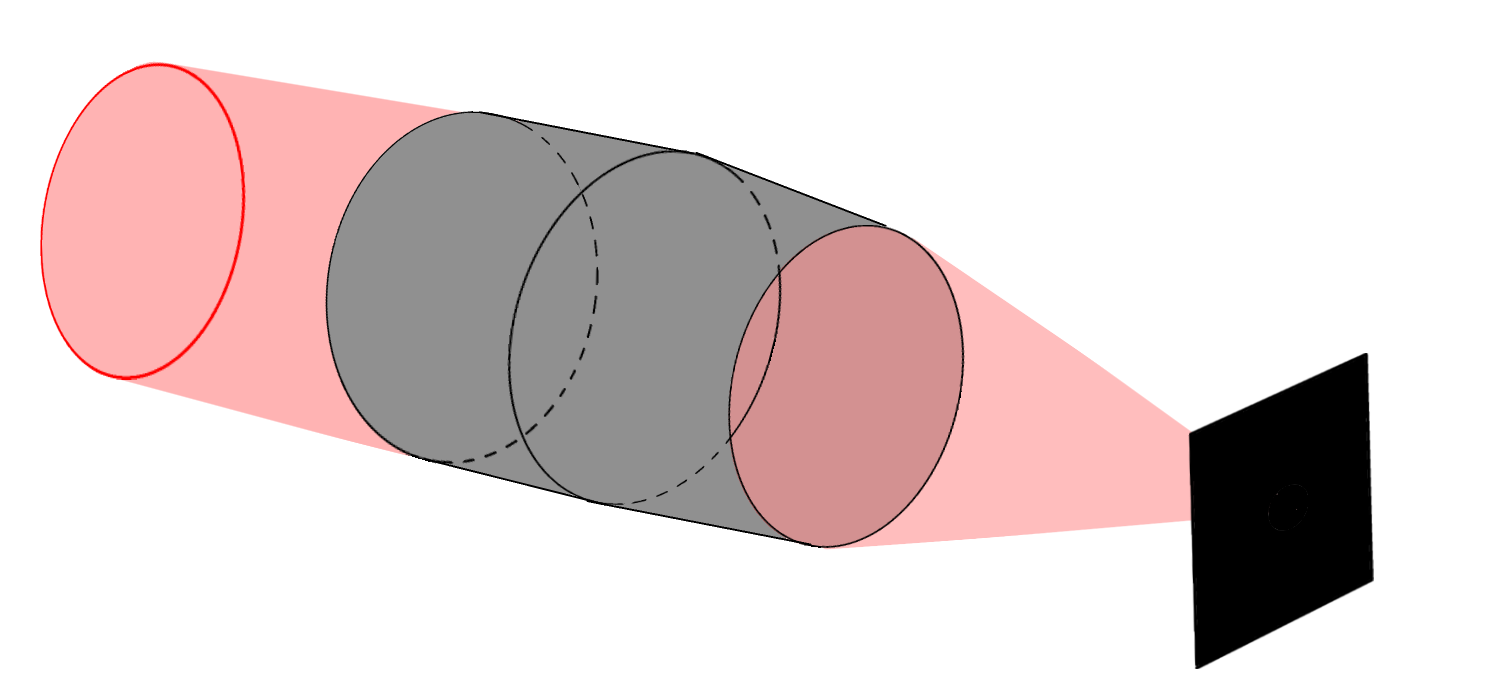
\includegraphics[width=12cm]{solitude_schematic_for_wolter.png}
\caption{Wolterミラー下流端面の孤立条件を用いる方法}
\label{fig:solitude_schematic}
\end{figure}

\subsection{タイコグラフィ法}
\label{chap3_ptychography_introduction}

\subsubsection{タイコグラフィ法の概要}
\ref{chap3_solitude_introduction}節では1枚の画像に対して孤立条件から冗長性を確保して位相回復を行ったが、タイコグラフィ法では光学系に徐々に変化を与えながら、多数の画像を撮影することによって冗長性を確保する。
図\ref{fig:ptychography_schematic}にその概要を示す。

\begin{figure}[!ht]
\centering
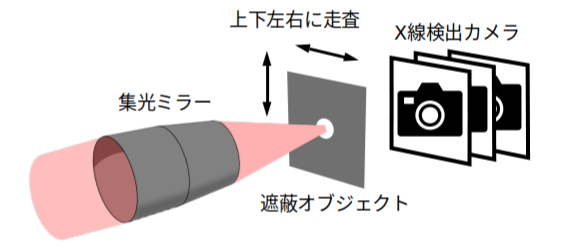
\includegraphics[width=12cm]{ptychography_schematic.png}
\caption{タイコグラフィ法の概要}
\label{fig:ptychography_schematic}
\end{figure}

集光ミラーに設計時に想定された光源からの入射光を入れ、その焦点面にオブジェクトを差し入れる。
このオブジェクトによって変化を受けた波面がさらに下流側に設置されたカメラによって撮影される。
これを、オブジェクトの位置を焦点面内で鉛直および水平方向に走査しながら多数の画像を撮影することで、冗長性を確保するという寸法である。
用いるオブジェクトは大きく分けて2種類ある。
1つはガラスなどの透過性を持つ物体の厚みに適当なパターンを与えた試料をオブジェクトとするものである。
物体の厚みを位置によって変えることで、それに応じて波面の位相の進み量に差が生じる。
試料の作製については、SiO2のエッチングによるパターニングなどが知られている。\cite{Godden2016}
この方法は、タイコグラフィによるミラー評価だけでなく、試料そのものを評価するタイコグラフィ顕微鏡としても利用できる。
もう1つは、ビームを完全に遮蔽できるような金属板に適当な穴を開けて作られるオブジェクトである。
焦点面における波面は完全に遮蔽される部分と完全に透過される部分の2つに分かれ、透過した波面の穴のエッジで回折した光が下流側のカメラに入射する。
これらのオブジェクトを焦点面内で走査し、各位置に対する回折光を

竹尾らは、ピンホール(1つの円形の穴)を開けた板をオブジェクトとして利用し、ピンホールのエッジをなぞるように走査する方法でタイコグラフィを行い、ミラー内面形状の評価に成功している。
ピンホールを用いた方法では、ミラーの内側で反射せず直接通過した光を処理することが位相パターンをつけた試料より容易である。

\subsubsection{PIE}
位相回復法は元来、X線顕微鏡として利用されたため、回復の対象はサンプル(オブジェクト)であった。
その最も簡単なタイコグラフィのアルゴリズムがPIE(Ptychography Iterative Engine)である。
これは、照明関数は既知であるとして与え、オブジェクトのみ回復計算を行うアルゴリズムである。
PIEの疑似コードをAlgorighm\ref{alg:pie}に示す。

\begin{algorithm}                      
\caption{PIE Algorithm}         
\label{alg:pie}                          
\begin{algorithmic}
    \STATE $O_0(\pos) = \mathrm{rand}(0,1) \exp(i \mathrm{rand}(0,1) )$
    \FOR{n = 0 \ldots N-1}
      \FOR{j = 0 \ldots M-1}
        \STATE $\psi(\pos_j) = P(\pos) O_n(\pos_j + \pos)$
        \STATE $\Psi(\rpos) = \mathcal F [\psi(\pos)]$
        \STATE $\Psi'(\rpos) = \sqrt{I_j(\rpos)} \exp\left( i \arg \psi(\pos) \right)$ 
        \STATE $\psi'(\pos) = \mathcal F^{-1} [\Psi'(\rpos)]$
        \STATE $O_{n+1}(\pos + \pos_j)'
          = O_n(\pos + \pos_j) 
          + \frac{P_n^*(\pos)}{|P(\pos)|^2+\varepsilon} \left( \psi_n'(\pos) - \psi_n(\pos) \right)$
      \ENDFOR
    \ENDFOR
\end{algorithmic}
\end{algorithm}

逆空間で拘束を掛け、実空間に戻したあとで、オブジェクトを更新する。
オブジェクトの更新則としてシンプルなのは$\psi(\pos_j) = P(\pos) O_n(\pos_j + \pos)$としたのに対応させて$O_{n+1}(\pos_j + \pos) = \frac{\psi'(\pos_j)}{P(\pos)}$とする方法である。
しかし、これは除算に際して発散が起こる可能性があり、実用上大きな問題を孕んでいる。
これを、式\ref{eqn:object_update_derivation}のように変形する。
\begin{eqnarray}
O_{n+1}(\pos_j + \pos)
  &=& \frac{\psi'(\pos_j)}{P(\pos)} \nonumber \\
  &=& \left( O_n(\pos_j + \pos) - \frac{\psi(\pos_j)}{P(\pos)} \right) + \frac{\psi'(\pos_j)}{P_n(\pos)} \nonumber \\
  &=& O_n(\pos_j + \pos) + \frac{1}{P(\pos)} \left( \psi'(\pos_j) - \psi(\pos_j) \right) \label{eqn:object_update_derivation}
\end{eqnarray}

これを一般化して文字を置き換えると、式\ref{eqn:object_update_simplified}のように書ける。
\begin{equation}
\label{eqn:object_update_simplified}
  O_{n+1}(\pos_j + \pos) = O_n(\pos_j + \pos) + w \Delta\psi(\pos)
\end{equation}
この更新の重み$w$を変えることで、アルゴリズムの改善を図る。
発散を回避するため、重みの分母を実数化して微小な定数$\varepsilon$を足して式\ref{eqn:pie_object_update_weight}のように重みを定めたのがAlgorithm\ref{alg:pie}に示したPIEのアルゴリズムである。
\begin{equation}
  \label{eqn:pie_object_update_weight}
  w = \frac{P^*(\pos)}{\left| P(\pos) \right|^2 + \varepsilon}
\end{equation}

\subsubsection{rPIE}
PIEがオブジェクトのみ回復を行っていたのに対して、照明関数も未知として回復計算を行うのがePIE(exteded PIE)である。
ePIEでは式\ref{eqn:pie_object_update_weight}のように定数で発散を回避するのではなく、式\ref{eqn:epie_object_update_weight}のように絶対値の2乗の最大値を取る。
また、更新係数にハイパーパラメタ$\alpha$を掛けることで収束性を上げることができることが知られている。
\begin{equation}
  \label{eqn:epie_object_update_weight}
  w = \alpha \frac{P_n^*(\pos)}{\max \left| P_n(\pos) \right|^2}
\end{equation}
ePIEでは照明関数も更新しなければいけないが、これはオブジェクトの更新と同様に式\ref{eqn:epie_probe_update}のように行われる。
\begin{equation}
\label{eqn:epie_probe_update}
  P_{n+1}(\pos) 
  = P_n(\pos) 
  + \beta \frac{O_n^*(\pos_j + \pos)}{\max \left| O_n(\pos_j + \pos) \right|^2} \Delta\psi(\pos)
\end{equation}

ePIE(式\ref{eqn:epie_object_update_weight})のように最大値を取る方法に対して、各点での絶対値の2乗とその最大値で重み付き平均を取って分母とするのがrPIE(regularized PIE)である。
更新式は式\ref{eqn:rpie_object_update}および式\ref{eqn:rpie_probe_update}に示す通りである。
rPIEはほとんどePIEの一般化になっている。
\begin{eqnarray}
  O_{n+1}(\pos_j + \pos) &=& O_n(\pos_j + \pos) 
    + \frac{P_n^*(\pos_j + \pos)}
      {\alpha \max \left| P_n(\pos) \right|^2 + (1-\alpha) \left| P_n(\pos) \right|^2}
    \Delta\psi(\pos) \label{eqn:rpie_object_update} \\
  P_{n+1}(\pos) &=& P_n(\pos) 
    + \frac{O_n^*(\pos_j + \pos)}
      {\beta \max \left| O_n(\pos_j + \pos) \right|^2 + (1-\beta) \left| O_n(\pos_j + \pos) \right|^2}
    \Delta\psi(\pos) \label{eqn:rpie_probe_update}
\end{eqnarray}

rPIEのアルゴリズムをAlgorithm\ref{alg:rpie}に示す。

\begin{algorithm}[!ht]
\caption{rPIE Algorithm}         
\label{alg:rpie}                          
\begin{algorithmic}
    \STATE $O_0(\pos) = \mathrm{rand}(0,1) \exp(i \mathrm{rand}(0,1) )$
    \STATE $P_0(\pos) = \mathrm{rand}(0,1) \exp(i \mathrm{rand}(0,1) )$
    \FOR{n = 0 \ldots N-1}
      \FOR{j = 0 \ldots M-1}
        \STATE $\psi(\pos_j) = P_n(\pos) O(\pos_j + \pos)$
        \STATE $\Psi(\rpos) = \mathcal F [\psi(\pos)]$
        \STATE $\Psi'(\rpos) = \sqrt{I_j(\rpos)} \exp\left( i \arg \psi(\pos) \right)$ 
        \STATE $\psi'(\pos) = \mathcal F^{-1} [\Psi'(\rpos)]$
        \STATE $O_{n+1}(\pos_j + \pos) 
          = O_n(\pos_j + \pos) + \frac{P_n^*(\pos_j + \pos)}
          {\alpha \max \left| P_n(\pos) \right|^2 + (1-\alpha) \left| P_n(\pos) \right|^2}
          \Delta\psi(\pos)$
        \STATE $P_{n+1}(\pos)
          = P_n(\pos) + \frac{O_n^*(\pos_j + \pos)}
          {\beta \max \left| O_n(\pos_j + \pos) \right|^2 + (1-\beta) \left| O_n(\pos_j + \pos) \right|^2}
          \Delta\psi(\pos)$
      \ENDFOR
    \ENDFOR
\end{algorithmic}
\end{algorithm}

タイコグラフィ法においても、走査ステップを変えることで回復領域の重なり具合が変化し、この比(オーバーサンプリング比)が収束性を左右する。
ステップが小さいほどオーバーサンプリング比は大きく収束性は高くなるが、その分必要な領域を走査し終えるのに必要な計測時間は増大してしまう。
Bunkらの検討によれば、オーバーサンプリング比が0.6程度が最適であるということが知られている。\cite{Bunk2008}

\subsection{ディテクター走査による冗長性}
\label{chap3_detector_scanninc_introduction}

タイコグラフィ法ではオブジェクトを走査することで冗長性を確保したが、ディテクターを走査することで冗長性を確保する方法も知られている。

\begin{figure}[!ht]
\centering
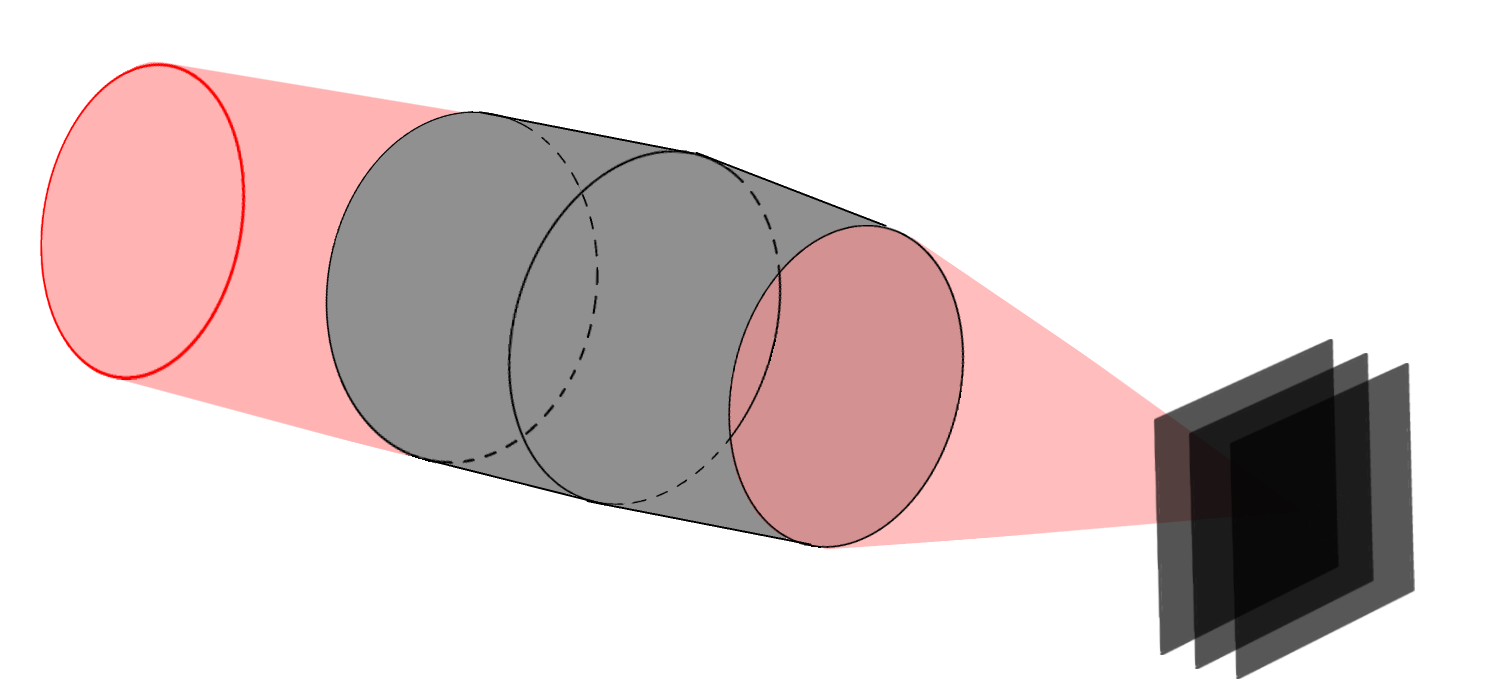
\includegraphics[width=12cm]{detector_scanning_schematic.png}
\caption{ディテクターを走査する方法の概要}
\label{fig:detector_scanning_schematic}
\end{figure}

下流端面から各ディテクター走査位置までの伝播計算は、焦点面までFresnel回折伝播、そこからさらに角スペクトル法でディテクター走査距離ぶんの伝播をするという2段階の構成で行われる。
タイコグラフィ法同様、各面に伝播するごとに強度を計測強度値と置き換える拘束を掛けることを繰り返し位相分布を回復する。

\subsection{下流端開口走査による冗長性}
\label{chap3_transverse_introduction}

オブジェクトを走査する位置を焦点面ではなく集光素子の開口直後とするTransverse Translation法がBradyらによって提案されている。\cite{Brady2009}
これは図\ref{fig:transverse_schematic}に示すように、焦点面を操作するタイコグラフィ法同様にオブジェクトを集光素子の開口で走査し、その回折像を下流側のカメラで撮影するという方法である。

\begin{figure}[!ht]
\centering
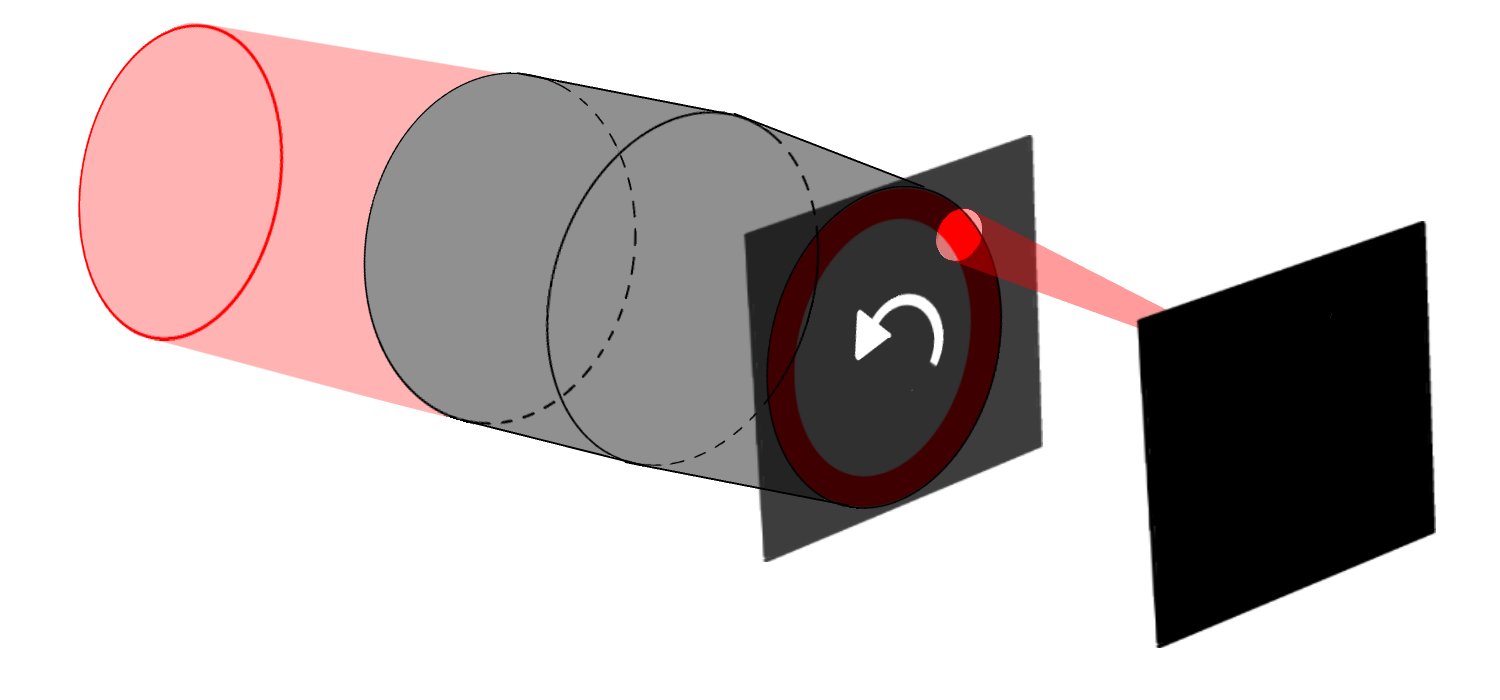
\includegraphics[width=12cm]{transverse_schematic.png}
\caption{Transverse Translation Diversityの概要}
\label{fig:transverse_schematic}
\end{figure}

輪帯はほぼ真円状になっているため、走査には回転ステージが有効である。
計算アルゴリズム自体は基本的にはタイコグラフィ法と同様にすればよく、特にピンホール形状の曲率誤差が問題にならない場合はピンホールは既知の円形状として与え、HIOとPIEを混合したアルゴリズムを用いればよい。

\clearpage
% ================================================== %
% section
% ================================================== %
\newpage

\section{手法の比較・決定}

\subsection{分解能に関する検討}
\label{chap3_comparison_resolution}

計測によって得られる下流端面の空間分解能を比較する上で最も重要なのは、位相回復計算の対象となる2つの平面がどこに設定されているかということである。
この観点で比較すると、上に挙げた4つの手法は孤立条件(\ref{chap3_solitude_introduction}節)、ディテクター走査(\ref{chap3_detector_scanninc_introduction}節)、下流端面走査(\ref{chap3_transverse_introduction})の3つと焦点面走査(\ref{chap3_ptychography_introduction})の2種類に大別される。
前者は下流端面と焦点面(近傍)におかれたCCD面、後者は焦点面に置かれたオブジェクト平面とそれよりさらに下流にあるCCDカメラの受光面が回復計算の対象となる。
\ref{chap3_sampling_theorem}節で述べたサンプリング定理に基づいて考えると、下流端面の空間分解能が高いことは焦点面における回復領域が大きいことに対応する。
前者の方法では、焦点面の回復領域の大きさはCCDカメラの受光面の大きさによって決まる。
\ref{chap3_dynamic_range}節に示したCCDを利用し、CCD全面に渡って回復計算を行うことができたとすれば、下流端面の1画素の一辺は\SI{32.66}{\micro \metre}であり、輪帯を動径方向に11.13ピクセルの分解能で計測できる。
一方で、後者の方法では焦点面の回復領域の大きさは走査面積によって決まり、その走査全体で必要となる撮影回数はCCDカメラの画素サイズによって決まる。
一方で焦点面走査の場合、1枚の画像に対応して回復される領域サイズはビームの焦点強度分布においてメインローブの数倍から10倍程度であり、前者と同じ36.9 mmの領域を回復するためには、10万枚オーダーの撮影が必要になる。
1枚の撮影に数秒程度かかるとすればこれは計測時間が現実的なものではなく、今回のWolterミラー計測には適さない。

\subsection{ダイナミックレンジに関する検討}
\label{chap3_comparison_dynamic_range}

続いて、焦点面にCCDカメラを配置する残り3つの手法について、ダイナミックレンジに関する検討を行う。
図\ref{fig:single_pinhole_mask}のように下流端面に$\Phi 4.5$ mmのピンホールを入れた場合、およびオブジェクトを何も挿入せず焦点面に光を集めた場合について、その集光面強度分布を図\ref{fig:comparison_focus_pinhole_existence}に示す。
また、水平方向プロファイルを強度ピークで規格化して比較したものが図\ref{fig:comparison_focus_pinhole_existence}である。
全面照明の場合は集光点付近に強度分布が集中しているのに対して、ピンホールを挿入すると広範囲に渡って分布していることが分かる。
このことから、ピンホールを挿入する方が、ダイナミックレンジに対応して有効領域が狭まるということが起きにくく、より安定した回復計算の収束が期待できる。

\begin{figure}[!ht]
\centering
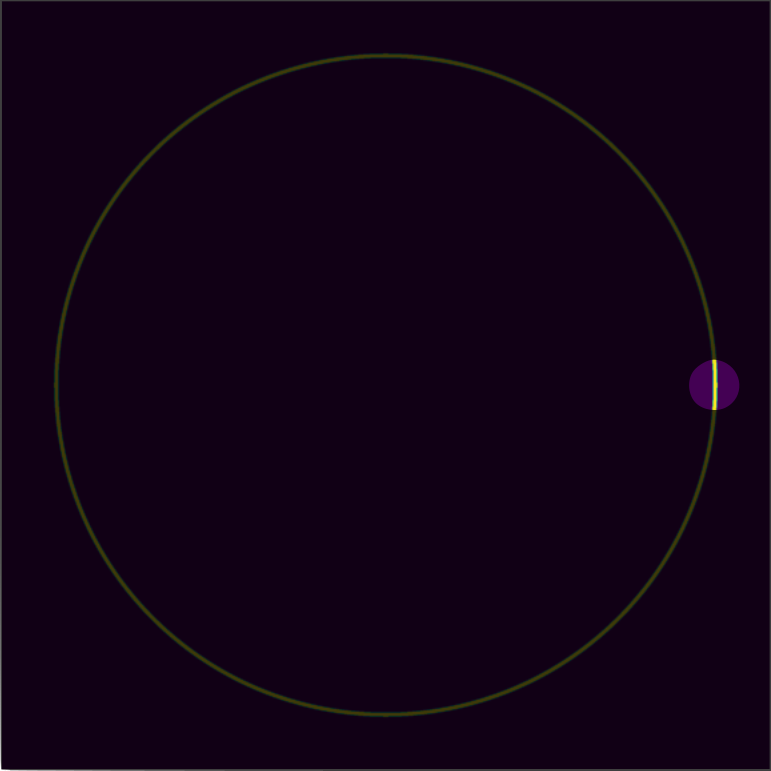
\includegraphics[width=6cm]{single_pinhole_masked_ring.png}
\caption{下流端面でのピンホールの模式図}
\label{fig:single_pinhole_mask}
\end{figure}


\begin{figure}[!ht]
\centering

\subfloat[オブジェクトがない場合]{
    
\includegraphics[width=6cm]{full_field_focus.png}
    \label{fig:full_field_focus}
}
\subfloat[$\Phi 4.5$ mmのピンホールを挿入した場合]{
    \centering
    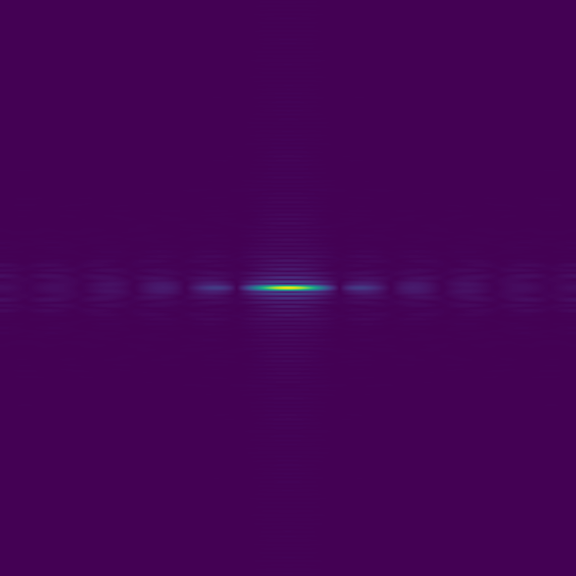
\includegraphics[width=6cm]{single_pinhole_focus.png}
    \label{fig:single_pinhole_focus}
}

\caption[]{ピンホールの有無による焦点面強度分布の比較}
\label{fig:comparison_focus_pinhole_existence}
\end{figure}

\begin{figure}[!ht]
\centering
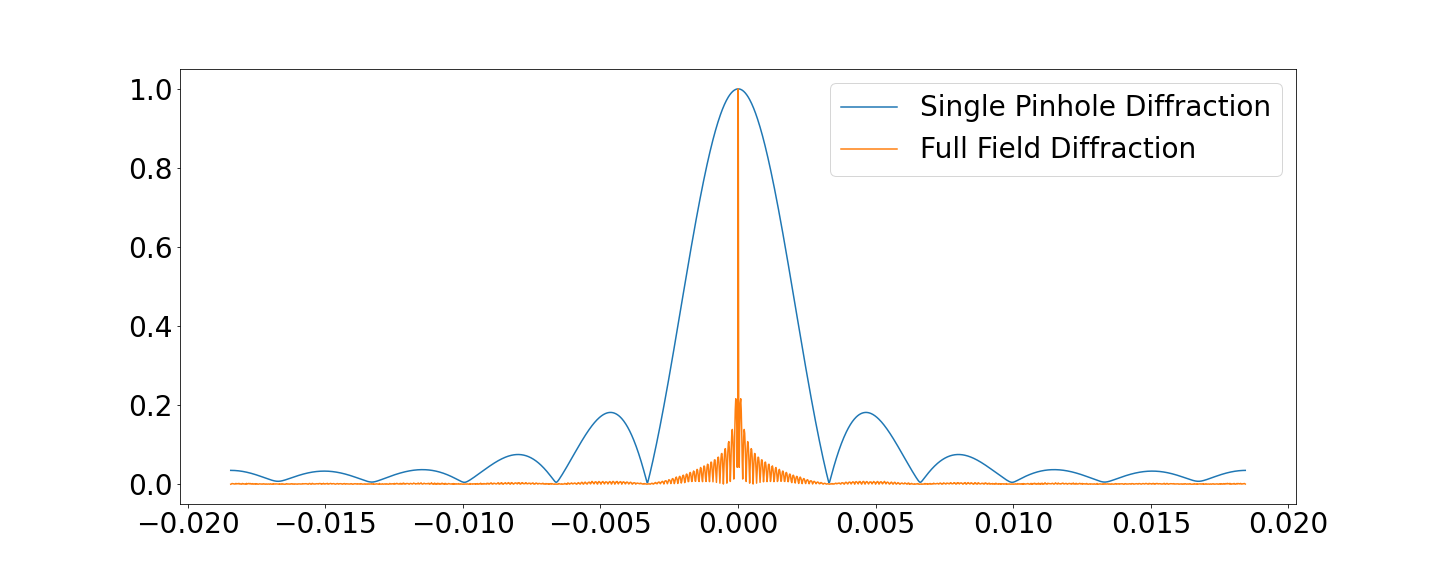
\includegraphics[width=14cm]{pinhole_dynamic_range_superiority.png}
\caption{ピンホールの有無による焦点面強度プロファイルの比較}
\label{fig:transverse_dynamic_range_superiority}
\end{figure}

\subsection{手法の選択}
\label{chap3_decision_of_method}
空間分解能に関する議論、およびダイナミックレンジに関する議論から、\ref{chap3_transverse_introduction}節の下流端に挿入したオブジェクトを走査する方法が最も安定して高い空間分解能での測定を実現すると結論づけ、これを測定手法として採用する。

\clearpage
% ================================================== %
% section
% ================================================== %
\newpage

\section{手法の提案}
\label{chap3_transverse_arrangement}

下流端開口面を走査する方法について、その構成を検討する。
\ref{chap3_comparison_dynamic_range}節で図\ref{fig:single_pinhole_focus}に示したように、ピンホールを挿入した際の理想的な輪帯に対して焦点面の強度分布は対称になっている。
つまり、輪帯上の半周ずれた点にピンホールを置いた場合と焦点面強度分布が変わらないため、焦点面における拘束が波面を解に近づけるとは限らない。
実際、\ref{fig:single_pinhole_mask}の構成において位相回復計算シミュレーションを行ったが、波面は正しく回復されなかった。
Bradyらの計測においては、焦点面よりも下流側にCCDカメラを配置することで非対称化を図っている。\cite{Brady2009}
例として、500 mm下流側における強度分布を角スペクトル法で計算すると図\ref{fig:single_pinhole_defocus}のようにデフォーカスし、対称性が崩れる。

\begin{figure}[!ht]
\centering
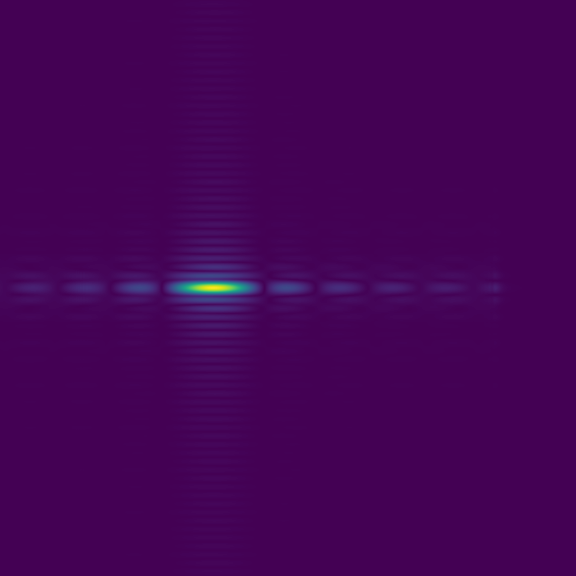
\includegraphics[width=6cm]{single_pinhole_defocus.png}
\caption{焦点面から500 mm下流側での強度分布}
\label{fig:single_pinhole_defocus}
\end{figure}

この方法の欠点として、焦点位置を調整したあとに移動を行うために位置決め精度が必要であること、回復計算ごとに線状畳み込みが必要な角スペクトル法での計算が必要となり計算時間が大きくなってしまうことが挙げられる。

\subsection{不等間隔複数ピンホールによる非対称化}
デフォーカスを用いない方法として、ピンホールを複数配置することで非対称性をもたせるという手法を提案する。
ピンホール2つでは、ピンホールが2つの場合と状況が変わらず、位相を回復することができない。
ピンホール2つを対称に配置し、さらにそこから角度をずらした位置にピンホールを配置することにより、非対称性を生み出すことができる。
図\ref{fig:three_pinhole_mask}はその一例として、対称な位置に2つとそこから45度ずれた位置にピンホールを挿入した場合について示した。

\begin{figure}[!ht]
\centering
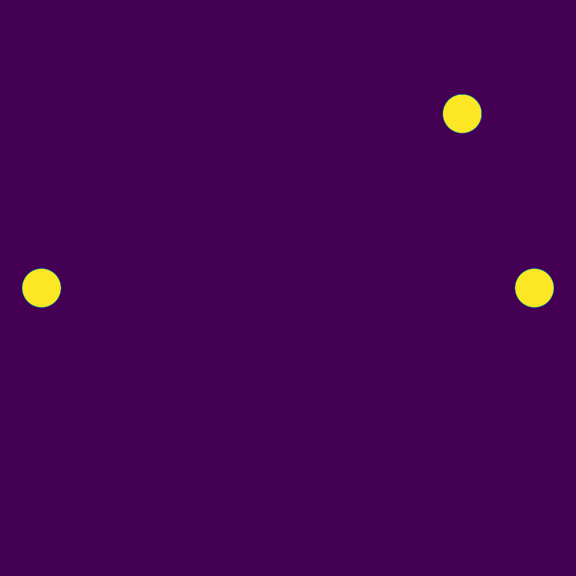
\includegraphics[width=6cm]{three_pinhole_mask.png}
\caption{不等間隔ピンホールの例}
\label{fig:three_pinhole_mask}
\end{figure}

このようにピンホールを配置すると、焦点面における強度分布は図\ref{fig:three_pinhole_focus}のようになる。

\begin{figure}[!ht]
\centering

\includegraphics[width=6cm]{three_pinhole_focus.png}
\caption{不等間隔ピンホールの例}
\label{fig:three_pinhole_focus}
\end{figure}

\clearpage
% ================================================== %
% section
% ================================================== %
\newpage

\section{適用するアルゴリズムに関する検討}
\label{chap3_algorithm}



\clearpage
% ================================================== %
% section
% ================================================== %
\newpage

\section{提案手法に関するシミュレーション}
\label{chap3_transverse_simulation}

本節では、まず位相回復計算およびシミュレーションに必要な光学波動場の伝播計算、および位相回復結果の解析に必要となる位相接続について述べた上で、提案手法についてシミュレーションを行い、その結果を示す。

\subsection{Wolterミラーにおける光学波動場の伝播}
\label{chap3_wolter_diffraction_apporoximation}
シミュレーションおよび位相回復計算を行うにあたり、測定対象のWolterミラーの光学系において適用するべき波動場伝播の近似公式について検討する。
光学波動場の伝播に関しての詳細は付録において解説する。
まず、1章\ref{chap1_wolter_arrangement}節で示したパラメータについて、Fresnel回折近似の成立条件が成り立っているかどうかを確認する。
Fresnel回折近似が成り立つための条件は、近似で切り捨てる微小項が1 radより十分小さいときであり、これは式\ref{eqn:fresnel_approximation_condition}で表される。
ただし$z$は伝搬距離、$\lambda$は波長、$(x, y), (\xi, \eta)$は実空間および逆空間の座標を表す。

\begin{equation}
\label{eqn:fresnel_approximation_condition}
    \frac{\pi}{4\lambda} \max \left\{ (x-\xi)^2 + (y-\eta)^2 \right\}^2 / z^3 \ll 1
\end{equation}

焦点面を3章\ref{chap3_dynamic_range}節に示したCCDカメラのサイズとして取りこれを計算すると、(左辺)の値は1.645 radとなった。
これは十分小さいとは言えず、Fresnel回折近似を満たしているとは言えない。
しかし、Fresnel回折近似を満たしていない場合でも、計算を進めていく上でそれがほとんど影響を及ぼさない場合がある。
位相回復計算においては数万回の伝搬計算を行うため、1回のコストは最小限であることが好ましい。
そこで、厳密計算であるRayleigh-Sommerfeld回折積分とFresnel回折積分近似の集光面強度分布を比較し、実用上の問題が存在するかどうかを検討する。
まず、表\ref{tb:check_approximation_validity_1}に示すような適当な分割で回折積分を実行し、集光波面分布におけるメインピークのFWHMを調べる。

\begin{table}[!ht]
\begin{center}
  \caption{Fresnel回折近似適用可能性の検討1}
  \begin{tabular}{|c|c|} \hline
    項目 & 値 \\ \hline
    波長 & 632.8 nm \\
    画素数 & $2048 \times 2048$ \\
    焦点面ピクセルサイズ & \SI{5.0}{\micro \metre} \\ \hline
  \end{tabular}
  \label{tb:check_approximation_validity_1}
\end{center}
\end{table}

計算の結果、プロファイルは図\ref{fig:fwhm_approximation}のようになった。

\begin{figure}[ht]
\centering
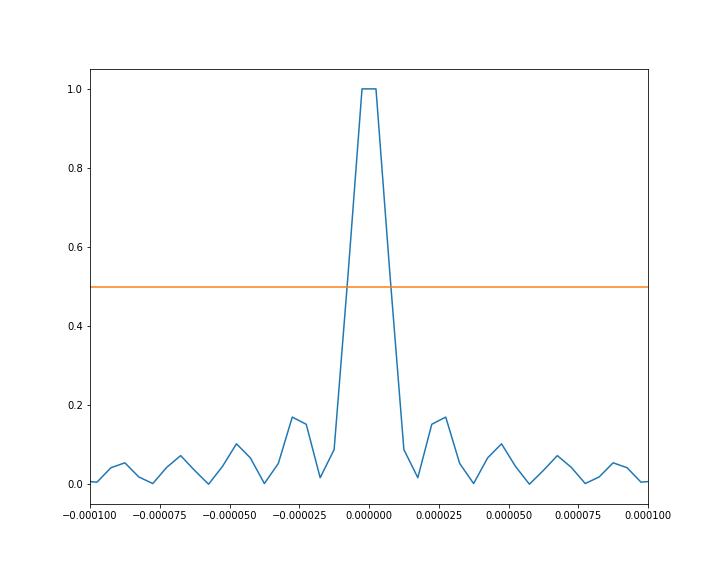
\includegraphics[width=8cm]{../../chap2/figure/fwhm_approximation.png}
\caption{回折積分計算による簡易的な計算で得られた焦点面強度プロファイル}
\label{fig:fwhm_approximation}
\end{figure}

ここから計算されるFWHMは4ピクセル分の\SI{20}{\micro \metre}であった。
これを踏まえ、メインピークを十分な分割数で観察できるよう焦点面ピクセルサイズが\SI{1}{\micro \metre}になるような表\ref{tb:check_approximation_validity_2}のパラメータで回折積分およびFresnel回折近似を用いた場合の集光面強度プロファイルを計算し、比較を行う。

\begin{table}[!ht]
\begin{center}
  \caption{Fresnel回折近似適用可能性の検討2}
  \begin{tabular}{|c|c|} \hline
    項目 & 値 \\ \hline
    波長 & 632.8 nm \\
    画素数 & $4096 \times 4096$ \\
    焦点面ピクセルサイズ & \SI{1.0}{\micro \metre} \\ \hline
  \end{tabular}
  \label{tb:check_approximation_validity_2}
\end{center}
\end{table}

計算の結果、プロファイルは図\ref{fig:diffraction_comparison}のようになった。
また、2つのプロファイルの差分を取って回折積分の最大値で規格化したグラフが図\ref{fig:diffraction_comparison_normalized_diff}である。

\begin{figure}[!ht]
\centering

\subfloat[プロファイルプロット]{
    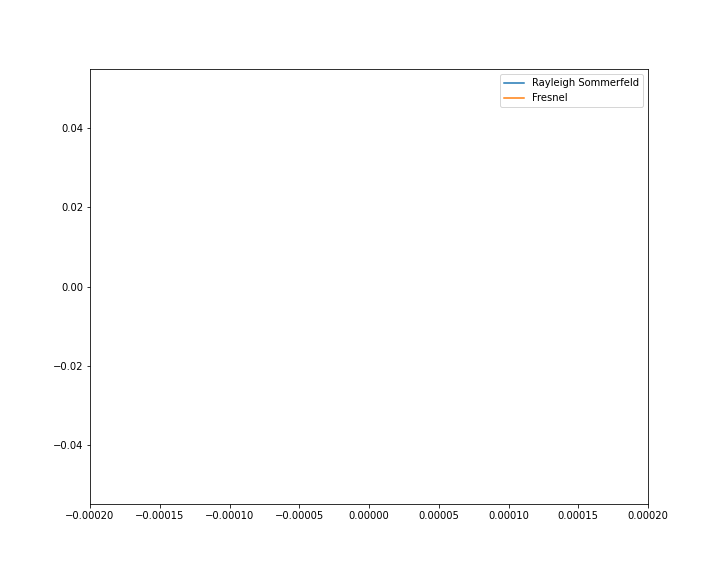
\includegraphics[width=6cm]{../../chap2/figure/diffraction_comparison_profile.png}
    \label{fig:diffraction_comparison_profile}
}
\subfloat[規格化されたプロファイル誤差]{
    \centering
    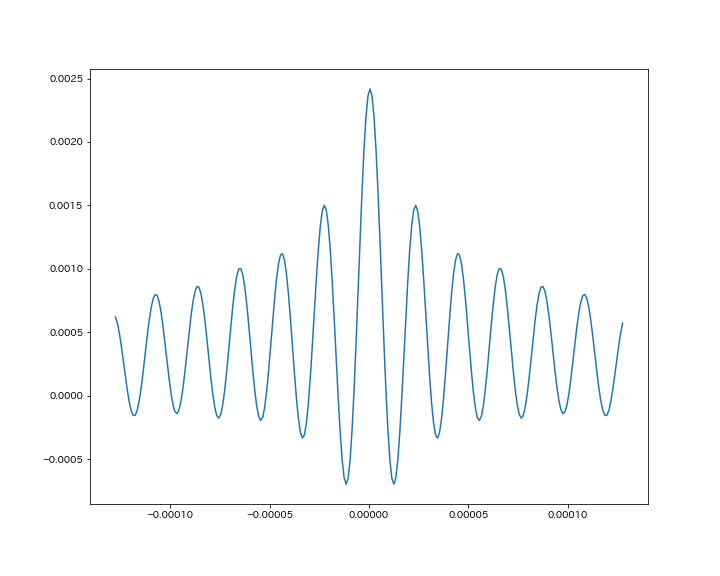
\includegraphics[width=6cm]{../../chap2/figure/diffraction_comparison_normalized_diff.png}
    \label{fig:diffraction_comparison_normalized_diff}
}

\caption[]{Rayleigh-Sommerfeld回折積分とFresnel回折積分のプロファイル比較}
\label{fig:diffraction_comparison}
\end{figure}

差分の絶対値の最大値は0.00242程度となった。
これは十分小さく、実際の計測で生じうるノイズと同程度以下であるため、シミュレーションでの検討および位相回復計算を行う上で致命的な問題をもたらさない。
ゆえに、以降の伝搬計算はFresnel回折近似を用いて行う。

\subsection{位相接続(位相アンラッピング)}
$\sin$関数などの周期関数は、逆関数の値域が周期以下の大きさしか持たないため、完全にもとの入力を戻すことはできない。
複素波動場の位相分布についても同様である。
$\exp(i\phi)$は周期$2\pi$の関数であり、逆関数は$\arg\{\exp(i\phi)\}=\phi \mod{2\pi}$と位相の$\mod{2\pi}$での剰余を返す。
故に、位相分布が本来なめらかな関数として与えられたとしても、それが$2\pi$を超えるような範囲に渡って分布する際には必ずどこかで不連続に位相が飛んでしまう。
例えば、$y = f(x) = 10x + 20x^2 \quad (x \in [0, 1])$に対して$z = \arg\{\exp(iy)\}$を取ると、図\ref{fig:wrapped_graph_example}のようになる。

\begin{figure}[ht]
\centering
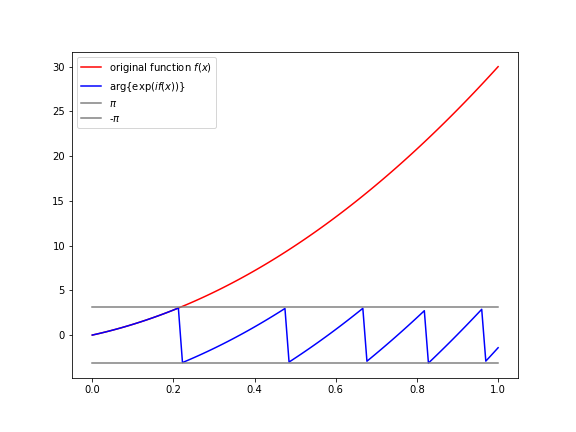
\includegraphics[width=10cm]{before_unwrap.png}
\caption{arg関数によって不連続になったグラフの例}
\label{fig:wrapped_graph_example}
\end{figure}

これに対して、離散化された領域において1ピクセルで$2\pi$以上のジャンプはないものと仮定して順番に接続を行うことで、なめらかな位相分布を取り戻すことができる。
これを位相接続あるいは位相アンラップといい、1次元の離散列$y[n] = f(x[n])$および$z[n]=\arg\{\exp(iy[n])\}$に対して最もシンプルなアルゴリズムはAlgorithm \ref{alg:unwrap_1d}のようになる。
連続した位置を走査していき、1つ前のピクセルと$\pi$以上の位相差が生じたらそれ以降の点全てに$2\pi$を足し引きし、位相を接続する。

\begin{algorithm}                      
\caption{1次元アンラップの例}         
\label{alg:unwrap_1d}                          
\begin{algorithmic}
    \FOR{$n = 1 \ldots N-1$}
        \STATE $\delta = \begin{cases}
                -2 \pi & (z[n] + \pi < z[n]) \\
                0 & (z[n] - \pi \leq z[n] \leq z[n] + \pi) \\
                2 \pi & (z[n] < z[n] - \pi)
            \end{cases}$
        \FOR{$k = n \ldots N-1$}
            \STATE $z[k] \leftarrow z[k] + \delta$
        \ENDFOR
    \ENDFOR
\end{algorithmic}
\end{algorithm}

2次元のリング状の領域に対しても同様にできる。
接続するべき2次元位相分布内においてその順序を決めれば、1次元の場合と同じアルゴリズムで接続を行うことができる。
本研究では、まず図\ref{fig:unwrap_transform}のように$x-y$座標から$\theta-r$の極座標分布に変換する。
その上で図\ref{fig:unwrap_path}のように$r$方向の中央部分を$\theta$方向に走査したのちにその各点から各$\theta$について動系方向に走査するといった順序でAlgorithm \ref{alg:unwrap_1d}を適用し、最後に$x-y$座標系に戻す。
ミラー波面計測においては、経験的に十分な空間分解能があれば$2\pi$以上のジャンプはないと考えてよいとされており、本研究でも同様にその仮定をおいて測定を行う。

\begin{figure}[!ht]
\centering
\subfloat[$x-y$座標における位相分布]{
    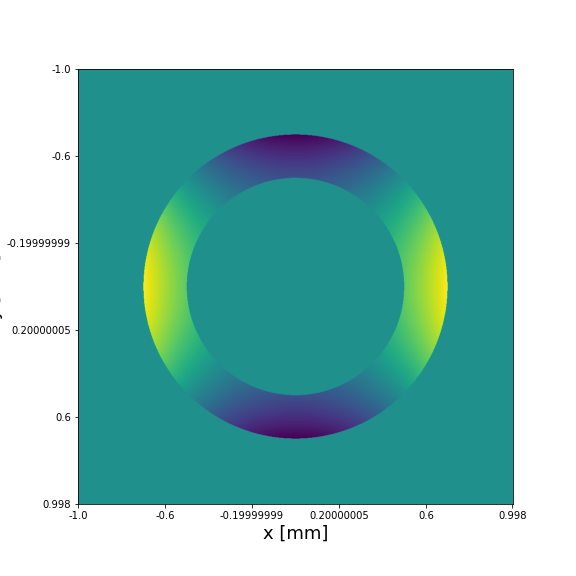
\includegraphics[width=6cm]{unwrap_xy.png}
    \label{fig:unwrap_xy}
}
\subfloat[極座標における位相分布]{
    \centering
    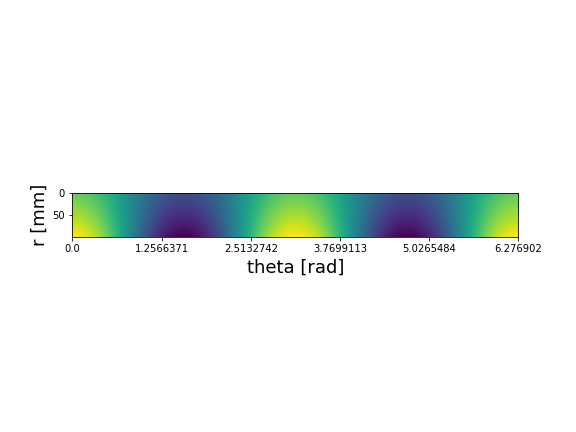
\includegraphics[width=6cm]{unwrap_polar.png}
    \label{fig:unwrap_polar}
}
\caption[]{位相分布の座標変換}
\label{fig:unwrap_transform}
\end{figure}

\begin{figure}[!ht]
\centering
\subfloat[$x-y$座標に対応させた走査経路]{
    \centering
    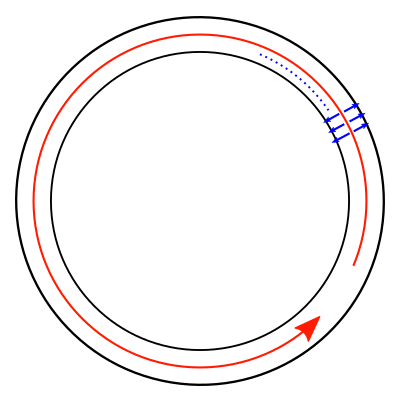
\includegraphics[width=6cm]{unwrap_path.png}
    \label{fig:unwrap_path_xy}
}
\subfloat[極座標での走査経路]{
    \centering
    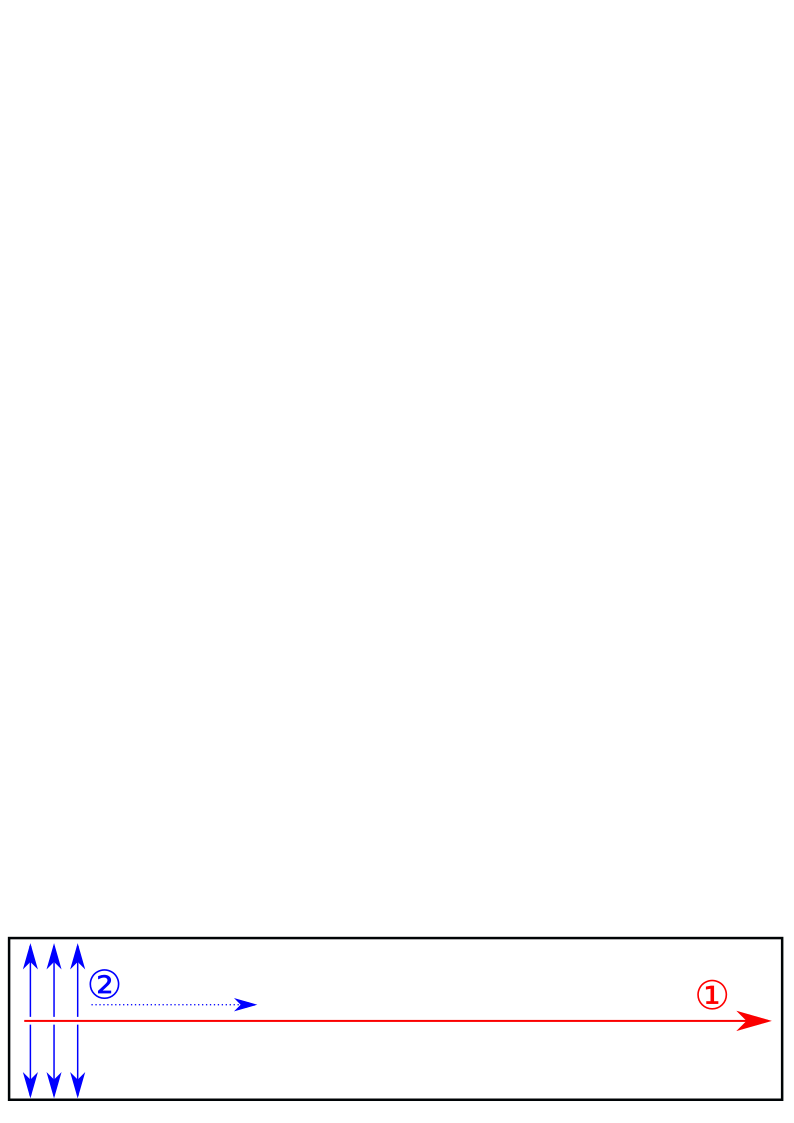
\includegraphics[width=6cm]{unwrap_path_polar.png}
    \label{fig:unwrap_path_polar}
}
\caption[]{位相分布の座標変換}
\label{fig:unwrap_path}
\end{figure}

\subsection{位相回復シミュレーションの結果}
\label{chap3_transverse_simulation_result}

現実の測定において現れる非点収差が存在する場合についてシミュレーション上の測定を行い、位相回復計算を行った。
図\ref{fig:sim_transverse}に入力波面および回復された波面を、また図\ref{fig:sim_profile_comparison}に輪帯幅の半分に当たる位置での周方向位相分布を比較したグラフを示す。
入力した位相分布に対して、回復計算が正しく収束し、波面が回復されていることが確認できる。

\begin{figure}[!ht]
\centering
\subfloat[入力した波面]{
    \centering
    
\includegraphics[width=6cm]{sim_answer.png}
    \label{fig:sim_answer}
}
\subfloat[回復された波面]{
    \centering
    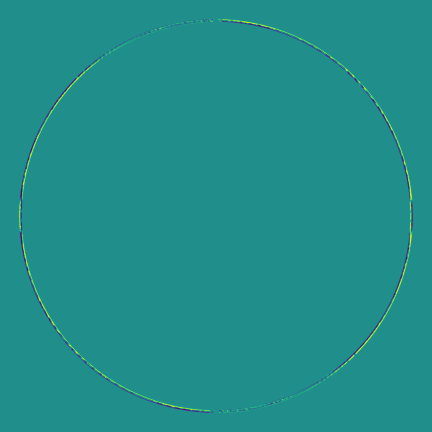
\includegraphics[width=6cm]{sim_reconstructed.png}
    \label{fig:sim_reconstructed}
}
\caption[]{位相回復シミュレーションの結果}
\label{fig:sim_transverse}
\end{figure}

\begin{figure}[ht]
\centering
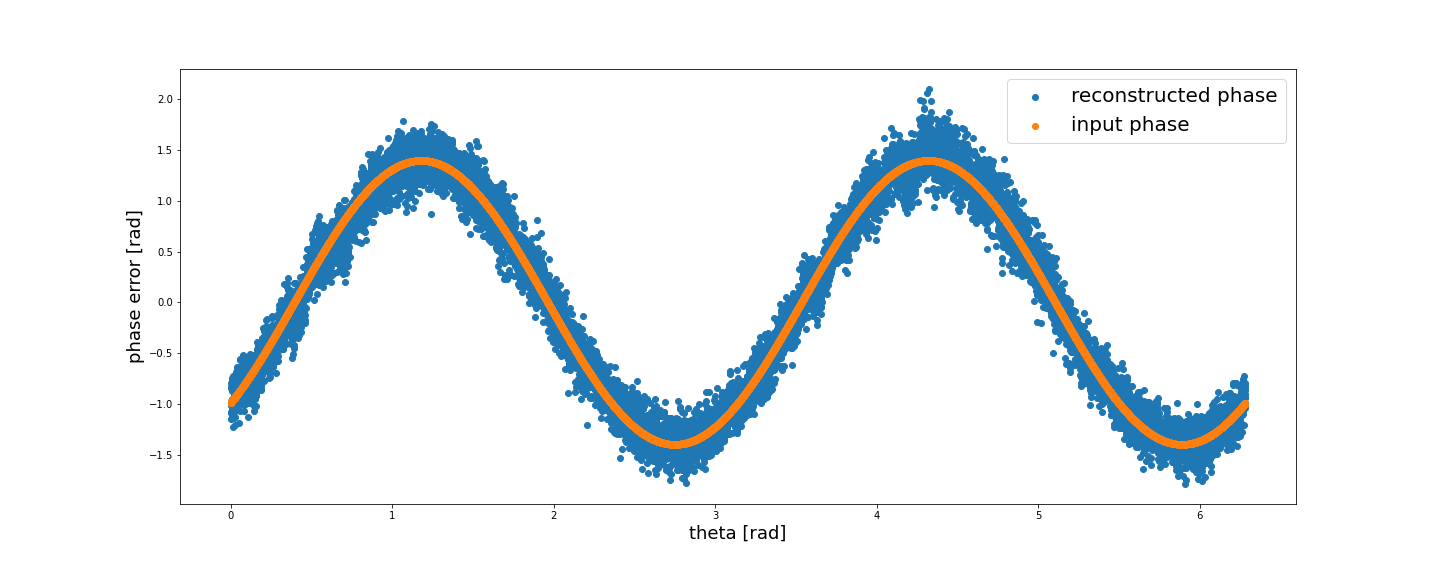
\includegraphics[width=10cm]{sim_profile_comparison.png}
\caption{回復波面と入力波面の輪帯中央でのプロファイル比較}
\label{fig:sim_profile_comparison}
\end{figure}

\clearpage
% ================================================== %
% section
% ================================================== %
\newpage

\section{計測波面以外の通過光の処理方法に関する検討}
\label{chap3_first_reflection_shutter}

測定対象となっている天文用Wolterミラーは、X線集光用に設計・作製されたものであり、可視光を入射した際にどのような集光波面が生じるかは未検討である。
\ref{chap3}章での提案手法の検討は、あくまで波面計測の対象である輪帯のみが存在する場合について行われたが、実際にミラーを計測する実験においては測定対象以外の光も通過してCCDカメラの方向に進行する。
円形の平行光を入射した際にミラーより下流に通過する光は、図\ref{fig:mirror_beam_path_types}に示す通り3種類存在する。
1つは計測対象の2回反射光、1つは放物面には当たらず双曲面で1回だけ反射された光、1つは直接通過光である。

\begin{figure}[!ht]
\centering
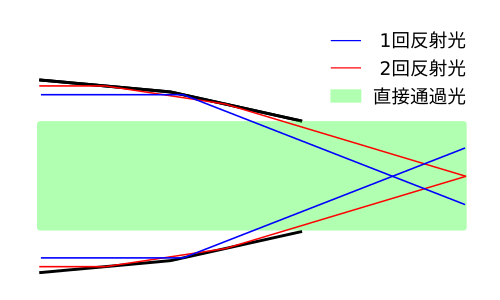
\includegraphics[width=10cm]{reflection_beam_types.png}
\caption{ミラーに入射した光の進路}
\label{fig:mirror_beam_path_types}
\end{figure}

直接通過光は、ピンホールの金属板によって遮蔽されており、またピンホールを通過してもCCDカメラの撮影領域から10 mm以上外れているためこれは計測強度値に影響を及ぼさない。
双曲面による一回反射光は、焦点面において直径約30 mmとなるため、CCDカメラに入射してしまう。
これを取り除く方法は2種類考えられる。
1つは、撮影される強度分布において1回反射光を含まない領域を切り出し、これを回復に用いる方法、もう1つは集光点より上流に存在する1回反射光の集まる位置でこれを遮蔽するという方法である。
前者では切り出しを行ったとしてもその回折光は入射してしまうほか、焦点面サイズを狭めることになるため下流端面の空間分解能が低下してしまう。
後者では集光ビームを遮ることなく遮蔽することはほとんど不可能である上、遮蔽板のエッジで回折した光はまた焦点面の強度分布に影響を及ぼしてしまう。
いずれも大きな問題を抱えているが、本実験では構成が簡単な前者を選択することとする。



\clearpage
% ================================================== %
% section
% ================================================== %
\newpage


\section{結言}
\label{chap3_conclusion}

位相回復法の中で空間分解能およびダイナミックレンジの観点から優れていると考えられる下流端面走査法について、非対称化の方法として不等間隔に穴を配置したオブジェクトの利用を提案した。
また、シミュレーションの結果から位相回復計算が正しく行われることを確認し、手法としての正当性を検証した。


%%%%%%%%%%%%%%%%%%%%%%%%%%%%%%%%%%%%%%%%%%%%%%%%%%%%%%%%%%%%%%%%%%%%%%%%%%%%%
%%% Local Variables:
%%% mode: katex
%%% TeX-master: "../thesis"
%%% End:
